\subsection{Anforderungen}

\subsubsection{Personas}
Unter der Definition von Personas\footcite{persona_definition} versteht man: 
\begin{displayquote}
Personas (lat. Maske) sind Nutzermodelle, die Personen einer Zielgruppe in ihren Merkmalen charakterisieren. Sie können z. B. einem Entwicklerteam aufgrund ihrer umfangreichen Beschreibung helfen, sich in die Lage der potenziellen Nutzer zu versetzen und diese Perspektive während des gesamten Designprozesses leicht zu vertreten. Sie werden mit einem Namen, einem Gesicht, einer Funktion, einem Werdegang und einem Privatleben versehen. Personas verfügen über Ziele und Verhaltensweisen, haben Vorlieben und Erwartungen.
\end{displayquote}

Diese Personas wurden erstellt, um ein klareres Bild vermitteln zu können, was die Anwendung genau ermöglicht.

\subsubsection*{Persona 1}
\subsubsection*{Persönliches Profil}
Abirsana ist Lehrerin an der Oberstufe Gossau und Unterrichtet die Fächer Mathematik, Deutsch und English.

\subsubsection*{Situation}
Um den Unterricht interessanter zu gestalten, greift Abirsana oft auf digitale Medien, wie zum Beispiel YouTube Videos, zurück. Oftmals ist jedoch das Material nicht genau auf den Schulstoff angepasst oder die Qualität lässt zu wünschen übrig.

\subsubsection*{Szenario}
Im Rahmen des Unterrichts soll es Abirsana möglich sein, die Aufgaben-Coaching Webanwendung zu verwenden. Sie soll in der Lage sein, einzelne Fächer und Theorieinhalte ihrer Klasse zur Verfügung zu stellen. Zudem kann sie eigene Übungen erfassen, welche die Schüler auch gleich über die Webanwendung lösen. Sind die Aufgaben abgegeben, kann sie die einzelnen Aufgaben anschauen und bewerten. Falls ihr auffällt, dass ein gewisser Schüler oder die ganze Klasse etwas nicht versteht, kann sie so direkt die Wissenslücke schliessen.

\subsubsection*{Persona 2}
\subsubsection*{Persönliches Profil}
Salina ist Schülerin an einer Schule. Seit längerer Zeit hat sie aber Mühe mit dem Schulstoff und ihre Noten sind auch nicht mehr so gut.

\subsubsection*{Situation}
Salina versteht oft nichts, wenn ihr Lehrer ihr etwas erklärt. Zu Hause verbringt sie dann viel Zeit im Internet, um einzelne Themen zu lernen. Sie hat aber weder die Zeit oder die Lust dazu, zu Hause nochmals die gesamte Theorie anschauen zu müssen.

\subsubsection*{Szenario}
Nach kurzer Zeit hat Salina die Lehrer an ihrer Schule dazu überredet, die Aufgaben-Coaching Plattform einzusetzen. Somit ist Salina freier im lernen. In der Schule kann sie sich selbstständig ein Thema beibringen. Falls sie dennoch etwas nicht versteht, kann sie direkt auf eine Lehrperson zugehen, welche ihr dann das Kapitel vielleicht noch etwas genauer erklärt. \\
Zudem wird sie nicht von anderen Schülern aufgehalten, weil diese länger brauchen, um ein Thema zu lernen.

\subsubsection*{Persona 3}
\subsubsection*{Persönliches Profil}
Liam ist der Informatik Verantwortliche an einer Schule. Er ist sehr Technik affin und sucht immer nach neuen Tools oder Programmen, welche in der Schule eingesetzt werden können.

\subsubsection*{Situation}
Seit geraumer Zeit regt er sich über die Lehrer auf, welche Jahr für Jahr das selbe erzählen und viel Geld dabei verdienen. Aus diesem Grund sucht er nach einer Lösung, wie die Lehrer trotzdem unterrichten können, aber nicht immer das gleiche erzählen.

\subsubsection*{Szenario}
Mit der Aufgaben-Coaching Webanwendung ist er auf ein Tool gestossen, welche genau das verspricht. Die ganzen Theorieeinheiten wurden bereits erfasst und stehen allen Lehrern zur Verfügung. Somit sparen die Lehrer viel Zeit bei der Vorbereitung, da bereits ein roter Faden durch den gesamten Stoff besteht. \\
Zudem kann Liam als Administrator die Statistiken einzelner Klassen anschauen. So kann er auch direkt sehen, wenn eine Klasse unter dem Durchschnitt der Schule ist und mehr Hilfe benötigt.


\subsubsection{Use Cases}

\subsubsection*{Use Case Diagramm}
\begin{minipage}{\textwidth}

\begin{figure}[H]
	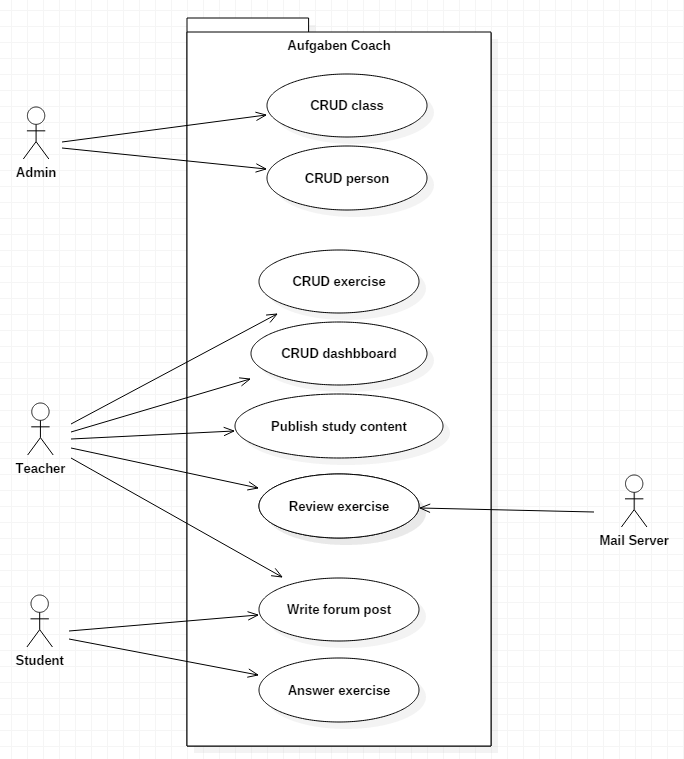
\includegraphics[width=\textwidth, height=\textheight, keepaspectratio]{images/UseCaseDiagramm.png}
	\caption{Use Case Diagramm}
\end{figure}

\end{minipage}


\begin{tabular}{| p{1cm} | p{1.3cm}|}
	\hline
	\textbf{Farbe} & \textbf{Priorität} \\
	\hline	
	grün & hoch \\
	\hline
	orange & tief \\
	\hline
\end{tabular}


\subsubsection*{Aktoren}

\begin{table}[H]
	\centering
	\begin{tabu} to 0.9\textwidth {l X}
	\toprule
	Aktor & Beschreibung \\ 
	\midrule
	Administrator & Der Administrator ist für die Verwaltung der Klassen, Lehrer und Schüler zuständig. Er kann Klassen erstellen sowie Lehrpersonen und Schüler diesen Klassen zuweisen \\
	\midrule
		Lehrer & Der Lehrer verwaltet die ihm zugewiesenen Klassen. Er kann Fächer für seine Klassen freischalten sowie Aufgaben erstellen und diese der Klasse zuweisen. Zusätzlich kann er Statistiken einsehen, die ihn über den aktuellen Wissensstand seiner Klasse informieren. \\
	\midrule
		Schüler & Die Schüler haben Zugriff auf freigeschaltete Lerninhalte und können diese anschauen. Falls Fragen auftreten, können diese im aufgaben-spezifischen Forum gestellt werden. Zusätzlich können Aufgaben gelöst werden. \\
	\bottomrule
	\end{tabu}
	\captionof{table}{Aktoren}
\end{table}


\subsubsection*{Beschreibung der Use Cases}
\textbf{UC01: CRUD person}

\noindent Hauptszenario: \\
Ein Administrator kann einen neuen Benutzer erstellen. Dabei kann er zwischen Lehrern und Schülern unterscheiden. Es müssen Angaben wie Vorname, Nachname, Benutzername, E-Mail Adresse und Passwort gemacht werden. Das System erstellt den gewünschten Benutzer, sodass dieser die Applikation ab sofort benutzen kann. \\

\noindent Alternatives Szenario: \\
Ein Administrator löscht eine nicht mehr berechtigte Person aus dem System. \\


\noindent \textbf{UC02: CRUD class}

\noindent Hauptszenario: \\
Ein Administrator erstellt eine neue Klasse. Dabei muss er den Namen der Klasse, wie auch das Eintrittsdatum angeben. Mit Hilfe des Eintrittsdatums kann im späteren Verlauf der Arbeit eine Statistik über mehrere ''Generationen'' von Klassen gemacht werden. \\

\noindent Alternatives Szenario: \\
Ein Administrator löscht eine nicht mehr benötigte Klasse aus dem System. \\


\noindent \textbf{UC03: assigne persons}

\noindent Hauptszenario: \\
Ein Administrator wählt eine bereits erstellte Klasse und weisst dieser eine unbestimmte Anzahl Lehrpersonen zu, sowie auch Schüler, welche noch keiner anderen Klasse zugewiesen wurden. \\

\noindent Alternatives Szenario: \\
Ein Administrator wählt eine bereits erstellte Klasse und entfernt Schüler und/oder Lehrer von dieser. \\


\noindent \textbf{UC04: CRUD exercise}

\noindent Hauptszenario: \\
Ein Lehrer definiert eine neue Aufgabe. Zur Aufgabe erstellt er mehrere Fragen. Zu jeder Frage kann er Hilfestellungen definieren, sowie angeben was die maximale Punktezahl ist. \\

\noindent Alternatives Szenario: \\
Ein Lehrer wählt eine erstellte Aufgabe aus und bearbeitet die Fragen dazu. Das heisst, es können weitere Fragen erstellt, bereits erstellte entfernt, oder aber auch neue Hilfestellungen hinzugefügt werden. \\


\noindent \textbf{UC05: CRUD weekly schedule}

\noindent Hauptszenario: \\
Ein Lehrer erstellt einen Wochenplan. Er erweitert Aufgaben und Quizzes mit einer Deadline und weisst diese einer seiner Klassen zu. \\

\noindent Alternatives Szenario: \\
Ein Lehrer bearbeitet einen bereits erstellten Wochenplan. Die Deadline einer Aufgabe wird um einen oder zwei Tage verschoben. \\


\noindent \textbf{UC06: CRUD quiz}

\noindent Hauptszenario: \\
Ein Lehrer definiert ein Quiz. Dazu erfasst er einige Fragen, die entsprechenden Antwortmöglichkeiten und die Lösungen. \\


\noindent \textbf{UC07: publish study content}

\noindent Hauptszenario: \\
Ein Lehrer schaltet ein neues Fach oder ein neues Thema für eine Klasse frei. \\

\noindent Alternatives Szenario: \\
Ein Lehrer entzieht einer Klasse das Recht ein Fach oder ein Thema zu sehen. \\


\noindent \textbf{UC08: view statistics}

\noindent Hauptszenario: \\
Ein Lehrer wählt eine Klasse und ein ihr zugewiesenes Fach aus. Das System berechnet anhand der von dieser Klasse gelösten Aufgaben eine Statistik und stellt diese dar. Wenn der Lehrer genauere Details sehen will, erstellt das System eine detailiertere Statistik. \\


\noindent \textbf{UC09: use forum}

\noindent Hauptszenario: \\
Ein Schüler sieht das aufgabenspezifische Forum. Findet er nicht die gewünschte Antwort, stellt er selber eine Frage. \\

\noindent Alternatives Szenario: \\
Ein Lehrer sieht, dass ein Schüler eine unbeantwortete Frage hat und beantwortet diese. \\


\noindent \textbf{UC10: send mail}

\noindent Hauptszenario: \\
Das System bemerkt, dass eine von einem Schüler gestellte Frage im Forum über längere Zeit nicht beantwortet wurde und informiert den Lehrer darüber per Mail. \\


\noindent \textbf{UC011: solve exercise}

\noindent Hauptszenario: \\
Ein Schüler löst eine Aufgabe. \\

\noindent Alternatives Szenario: \\
Ein Schüler überarbeitet eine bereits gelöste Aufgabe. \\


\noindent \textbf{UC012: solve quiz}

\noindent Hauptszenario: \\
Ein Schüler löst ein Quiz. \\

\noindent Alternatives Szenario: \\
Ein Schüler überarbeitet ein bereits gelöstes Quiz. \\


\subsubsection{Nicht Funktionale Anforderungen}
Bei der Erstellung der einzelnen \gls{nfr} wird auf FURPS zurückgegriffen. FURPS ist ein Akronym für Functionality, Usability, Reliability, Performance und Supportability. Dieses Modell wurde im Jahre 1992 von HP entwickelt und dient zur Priorisierung der Software Requirements.\footcite{furps_description}

\begin{table}[h]
	\centering
	\begin{tabu} to 0.9\textwidth {l l X}
	\toprule
	FURPS & Titel & Beschreibung \\ 
	\midrule
	Functionality & User Interface & Das User Interface der Applikation ist über den Webbrowser erreichbar. \\ 
	& Security & Die einzelnen Benutzer können nur auf die für sie freigegebenen Inhalte zugreifen. \\
	& HTTPS & Die Kommunikation zum Webserver soll über HTTS laufen. \\
	\midrule
	Usability & Responsiveness & Für Schüler soll die Applikation sowohl auf Desktop PCs wie auch auf Tablets oder Mobile Phones verfügbar sein. \\
	\midrule
	Reliability & Availability & Die Applikation soll 24/7 verfügbar sein. \\
	 & Fault Tolerance & Die Applikation soll bei unerlaubten Anfragen weiterhin verfügbar sein. \\
	\midrule
	Performance & Response Time & Wechselt der Benutzer zwischen einzelnen Seiten, soll die neue Seite in maximal einer Sekunde geladen worden sein.\\
	\midrule
	Supportability & Maintainability & Die Applikation soll gebaut werden, dass sie auch in Zukunft gewartet und ausgebaut werden kann. \\
	 & Scalability & Die Applikation soll von 300 Benutzern zeitgleich verwendet werden. \\
	\bottomrule
	\end{tabu}
	\captionof{table}{Non Functional Requirements}
\end{table}

%\subsubsection{Functionality}
%\subsubsection*{}
%
%\subsubsection{Qualität}
%Um die Qualität des Codes möglichst hoch zu halten und sicherzustellen, dass alle Teammitglieder immer auf dem aktuellsten Stand sind, werden auf Git Pull-Requests verwendet. Dadurch kann sichergestellt werden, dass ein anderes Teammitglied den geschriebenen Code ebenfalls angesehen und durchdacht hat.
%
%\subsubsection*{Maintainability}
%Die Software könnte unter Umständen in einem Start-Up verwendet werden. Da in Zukunft noch beinahe beliebig viele neue Anforderungen hinzustossen können, soll die Applikation so gebaut werden, dass sie einfach modifiziert werden kann. 
%
%\subsubsection*{Reliability}
%Die Applikation soll robust und reibungslos laufen, auch wenn mehere Schüler zeitgleich mit der Plattform verbunden sind.
%
%\subsubsection*{Scalability}
%Das System soll problemlos von bis zu 300 Benutzern gleichzeitig verwendet werden können. 
%
%\subsubsection*{Usability}
%Bei der Applikation soll es sich um eine Mobile First Applikation handeln. Die Plattform soll sowohl auf Desktop PCs, Tablets und Smartphones bedienbar sein. Der Lehrer- und Administator-spezifische Teil der Applikation ist davon erstmals ausgenommen, da davon ausgegangen wird, dass diese beiden Aktoren hauptsächlich auf Desktop PCs arbeiten. 
%Die Applikation soll ein intuitives User Interface besitzen, damit sich die Benutzer auf Anhieb zurechtfinden. 
%
%\subsubsection*{Security}
%Der Zugriff auf das System ist passwortgeschützt. Benutzer können sich nicht selbstständig registrieren. Nur Administratoren können neue Benutzer erfassen.
%Jede Person sieht nur die Informationen, die für sie selbst von Bedeutung sind. Ein Schüler hat zum Beispiel keinen Zugriff auf die Statistiken anderer Schüler.


\newpage